\begin{thema}{Β}
Στο παρακάτω σχήμα βλέπουμε τη γραφική παράσταση της \textbf{{παραγώγου}} $f'$ μιας συνάρτησης $f$, η οποία είναι παραγωγίσιμη στο $\mathbb{R}$.
\begin{center}
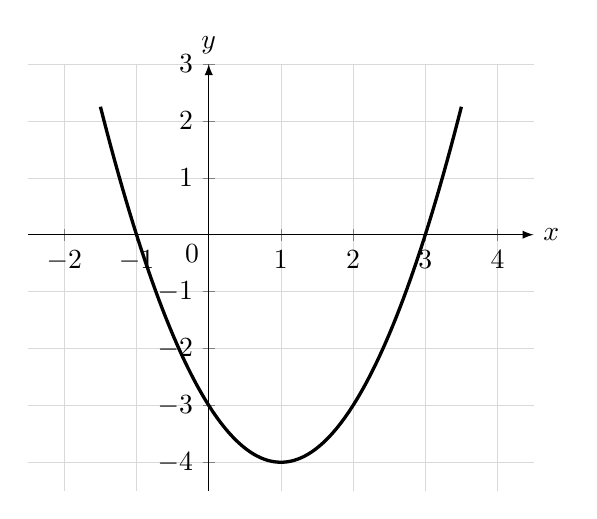
\begin{tikzpicture}
    \begin{axis}[axis lines = middle,
        axis line style = {->, >=latex},
        grid = major,
        grid style = {very thin, gray!30},
        xlabel = {$x$},
        ylabel = {$y$},
        xtick = {-2,-1,1,2,3,4,5},
        ytick = {-4,-3,-2,-1,1,2,3},
        every axis x label/.style = {at={(current axis.right of origin)}, anchor=west},
        every axis y label/.style = {at={(current axis.above origin)}, anchor=south},
        width = 8cm, height = 7cm, samples = 100,
        xmin=-2.5, xmax=4.5, ymin=-4.5, ymax=3,
        xtick distance=1, ytick distance=1
    ]
        \addplot[very thick, \xrwma, domain=-1.5:3.5] {x^2 - 2*x - 3};
        \node[below left] at (axis cs:0,0) {$0$};
    \end{axis}
\end{tikzpicture}
\end{center}
Με βάση το σχήμα:
\begin{erwthma}
  \item Να μελετήσετε τη συνάρτηση $f$ ως προς τη μονοτονία.
  \item Να βρείτε τις θέσεις και το είδος των τοπικών ακροτάτων της $f$.
  \item Να μελετήσετε τη συνάρτηση $f$ ως προς την κυρτότητα και τα σημεία καμπής.
  \item Αν επιπλέον γνωρίζετε ότι $f(0) = 2$, να βρείτε την εξίσωση της εφαπτομένης της $C_f$ στο σημείο της με τετμημένη $x_0=0$.
\end{erwthma}
\end{thema}
